%%%%%%%%%%%%%%%%%%%%%%%%%%%%%%%%%%%%%%%%%%%%%%%%%%%%%%%%%%%%%%%%%%%%%%%%%%%%%%%%%%%%%%%%%%%%%%%%%%%%
% Masters Thesis: A Deep Recurrent Network for Traffic Prediction
% Author: Rabindra Panda
% The University of Melbourne
%%%%%%%%%%%%%%%%%%%%%%%%%%%%%%%%%%%%%%%%%%%%%%%%%%%%%%%%%%%%%%%%%%%%%%%%%%%%%%%%%%%%%%%%%%%%%%%%%%%%

%---------------------------------------------------------------------------------------------------
%	PACKAGES AND OTHER DOCUMENT CONFIGURATIONS
%---------------------------------------------------------------------------------------------------

% The default font size and one-sided printing (no margin offsets)
\documentclass[11pt, oneside]{Thesis}

% Specifies the directory where pictures are stored
\graphicspath{{Pictures/}}
% Use the natbib reference package - read up on this to edit the reference style; if you want text
% (e.g. Smith et al., 2012) for the in-text references (instead of numbers), remove 'numbers'
\usepackage[square, numbers, comma, sort&compress]{natbib}
\usepackage{tikz}
\usetikzlibrary{trees,shapes,arrows,matrix,chains,positioning,decorations.pathreplacing}

% Colors hyperlinks in blue - change to black if annoying
\hypersetup{urlcolor=blue, colorlinks=true}
\title{\ttitle} % Defines the thesis title - don't touch this

\begin{document}

\frontmatter % Use roman page numbering style (i, ii, iii, iv...) for the pre-content pages

\setstretch{1.3} % Line spacing of 1.3

% Define the page headers using the FancyHdr package and set up for one-sided printing
\fancyhead{} % Clears all page headers and footers
\rhead{\thepage} % Sets the right side header to show the page number
\lhead{} % Clears the left side page header

\pagestyle{fancy} % Finally, use the "fancy" page style to implement the FancyHdr headers

\newcommand{\HRule}{\rule{\linewidth}{0.5mm}} % New command to make the lines in the title page

% PDF meta-data
\hypersetup{pdftitle={\ttitle}}
\hypersetup{pdfsubject=\subjectname}
\hypersetup{pdfauthor=\authornames}
\hypersetup{pdfkeywords=\keywordnames}

%---------------------------------------------------------------------------------------------------
%	TITLE PAGE
%---------------------------------------------------------------------------------------------------

\begin{titlepage}
\begin{center}

\textsc{\LARGE \deptname}\\ % Department name
\textsc{\LARGE \univname}\\[1.5cm] % University name
\textsc{\Large Masters Thesis}\\[0.5cm] % Thesis type

\HRule \\[0.4cm] % Horizontal line
{\huge \bfseries \ttitle}\\[0.4cm] % Thesis title
\HRule \\[1.5cm] % Horizontal line

\begin{minipage}{0.4\textwidth}
\begin{flushleft} \large
\emph{Author:}\\
% Author name
\href{http://www.rabipanda.com}{\authornames}
\end{flushleft}
\end{minipage}
\begin{minipage}{0.4\textwidth}
\begin{flushright} \large
\emph{Supervisor:} \\
% Supervisor name - remove the \href bracket to remove the link
\href{http://www.cis.unimelb.edu.au/people/staff.php?person_ID=618008}{\supname}
\end{flushright}
\end{minipage}\\[3cm]

 % University requirement text
\large \textit{A thesis submitted in fulfilment of the requirements\\ for the degree of
\degreename}\\[0.3cm]

%\textit{in the}\\[0.4cm]
%\groupname\\
%\deptname\\[2cm] % Research group name and department name

{\large \today}\\[4cm] % Date
%\includegraphics{Logo} % University/department logo - uncomment to place it

\vfill
\end{center}

\end{titlepage}

%---------------------------------------------------------------------------------------------------
%	DECLARATION PAGE
%---------------------------------------------------------------------------------------------------

\Declaration{

\addtocontents{toc}{\vspace{1em}} % Add a gap in the Contents, for aesthetics

I , \authornames, certify that

\begin{itemize}

\item[\tiny{$\blacksquare$}] this thesis does not incorporate without acknowledgement any material
previously submitted for a degree or diploma in any university; and that to the best of my knowledge
and belief it does not contain any material previously published or written by another person where
due reference is not made in the text.

\item[\tiny{$\blacksquare$}] the thesis is approximately 20000 words in length (excluding text in
images, table, bibliographies and appendices).
\end{itemize}

Signed:\\
\rule[1em]{25em}{0.5pt} % This prints a line for the signature

Date:\\
\rule[1em]{25em}{0.5pt} % This prints a line to write the date
}

\clearpage % Start a new page


%---------------------------------------------------------------------------------------------------
%	ABSTRACT PAGE
%---------------------------------------------------------------------------------------------------

\setstretch{1.3} % Reset the line-spacing to 1.3 for body text (if it has changed)

\abstract{\addtocontents{toc}{\vspace{1em}} % Add a gap in the Contents, for aesthetics

% Road traffic congestion as a global issue

% Adaptive traffic control systems and their role in mitigating the traffic congestion problem

% Short term traffic prediction and traffic loop data

% Time series anlysis for short term traffic prediction

% Neural networks and their reemergence as a victor

% Recurrent and LSTM networks

% Application
In this thesis we apply extend an LSTM model for the application of short term traffic flow
prediction. We analyse it using the SCATS volume data and suggest improvements.


}
\clearpage % Start a new page

%---------------------------------------------------------------------------------------------------
%	ACKNOWLEDGEMENTS
%---------------------------------------------------------------------------------------------------

\setstretch{1.3} % Reset the line-spacing to 1.3 for body text (if it has changed)

\acknowledgements{\addtocontents{toc}{\vspace{1em}} % Add a gap in the Contents, for aesthetics

I am deeply indebted to the following people for their invaluable support and comments without which
I would not have been able to complete this work\ldots
}
\clearpage % Start a new page

%---------------------------------------------------------------------------------------------------
%	LIST OF CONTENTS/FIGURES/TABLES PAGES
%---------------------------------------------------------------------------------------------------
% The page style headers have been "empty" all this time, now use the "fancy" headers as defined
% before to bring them back
\pagestyle{fancy}

\lhead{\emph{Contents}} % Set the left side page header to "Contents"
\tableofcontents % Write out the Table of Contents

\lhead{\emph{List of Figures}} % Set the left side page header to "List of Figures"
\listoffigures % Write out the List of Figures

\lhead{\emph{List of Tables}} % Set the left side page header to "List of Tables"
\listoftables % Write out the List of Tables

%---------------------------------------------------------------------------------------------------
%	ABBREVIATIONS
%---------------------------------------------------------------------------------------------------

\clearpage % Start a new page

\setstretch{1.5} % Set the line spacing to 1.5, this makes the following tables easier to read

\lhead{\emph{Abbreviations}} % Set the left side page header to "Abbreviations"
\listofsymbols{ll} % Include a list of Abbreviations (a table of two columns)
{
\textbf{ARIMA} & \textbf{A}uto \textbf{R}egressive \textbf{I}ntegrated \textbf{M}oving \textbf{A}verage \\
\textbf{LSTM} & \textbf{L}ong \textbf{T}erm \textbf{S}hort \textbf{M}emory \\
\textbf{RNN} & \textbf{R}ecurrent \textbf{N}eural \textbf{N}etwork \\
\textbf{SCATS} & \textbf{S}ydney \textbf{C}oordinated \textbf{A}daptive \textbf{T}raffic \textbf{S}ystems \\
}

%---------------------------------------------------------------------------------------------------
%	NOTATIONS
%---------------------------------------------------------------------------------------------------

%\clearpage % Start a new page
%
%\lhead{\emph{Notations}} % Set the left side page header to "Notations"
%
%\listofnomenclature{ll} % Include a list of Symbols (a two column table)
%{
%% Symbol & Name \\
%$y$ & Scalar value \\
%$\textbf{x}$ & Vector \\
%$\textbf{M}$ & Matrix \\
%$\Sigma$ & Covariance matrix \\
%}

%---------------------------------------------------------------------------------------------------
%	DEDICATION
%---------------------------------------------------------------------------------------------------

\setstretch{1.3} % Return the line spacing back to 1.3

\pagestyle{empty} % Page style needs to be empty for this page

\dedicatory{Dedicated to\ my parents}% Dedication text

\addtocontents{toc}{\vspace{2em}} % Add a gap in the Contents, for aesthetics

%---------------------------------------------------------------------------------------------------
%	THESIS CONTENT - CHAPTERS
%---------------------------------------------------------------------------------------------------

\mainmatter % Begin numeric (1,2,3...) page numbering

\pagestyle{fancy} % Return the page headers back to the "fancy" style

% Include the chapters of the thesis as separate files from the Chapters folder Uncomment the lines
% as you write the chapters


% Chapter 1

\chapter{Introduction} % Main chapter title

\label{Chapter1} % For referencing the chapter elsewhere, use \ref{Chapter1}

% This is for the header on each page - perhaps a shortened title
\lhead{Chapter 1. \emph{Introduction}}

% Quotation
{``As a reader I loathe introductions...Introductions inhibit pleasure, they kill the joy of
anticipation, they frustrate curiosity."}
\begin{flushright}
Harper Lee, \textit{To Kill a Mockingbird} (1960)
\end{flushright}

\section{Background}
Road traffic congestion is a serious global issue, resulting in significant wastage of resources.
While improving and extending the road infrastructure has reduced the issue to some extent, this is
time consuming and limited. Thus in last few decades, for better planning and control of road
traffic, adaptive traffic control systems have been deployed around the world. Still the role of
adaptive control systems is not fully realised without predictive capabilities in the short term. A
lot of research has gone into proposing short term traffic prediction models, yet none of those
models can be claimed to be perfect due to the nature of traffic data and the variable factors that
affect it.

\section{Objectives and scope}

\textbf{Research objective} is to propose a new model that can use the large amount of available
traffic data to predict the traffic in the short term. More importantly this research tries to answer the following questions -

\begin{itemize}
\item Can we design a deep neural network for traffic flow prediction.
\item Are we confident that the proposed model is better than existing models?
\end{itemize}

\textbf{Research scope} - There are several traffic characterstics that can be predicted such travel time and traffic volume. The scope of this research is limited to only traffic volume. While doing so, we are only taking the past data into consideration and ignoring other external factors such as weather, public events etc.


\section{Thesis outline}

\textbf{Chapters} -- This thesis is divided into six chapters.

\begin{itemize}
\item Chapter 1: Introduction - In this chapter we present the background and research context,
research objectives and scope.

\item Chapter 2: Traffic Prediction: Literature Review - In this chapter we review
the past research done in the area of short-term traffic flow forecasting.

\item Chapter 3: SCATS Traffic Volume Data - In this chapter we present the traffic volume data
collected by VicRoads using the SCATS volume data.

\item Chapter 4: A Deep Recurrent Network for Traffic Flow Prediction - In this chapter we propose a model that can be used in forecasting short-term traffic flow.

\item Chapter 5: Evaluation of the Model - In this chapter we evaluate the model.

\item Chapter 6: Conclusions and Future Directions - Finally we conclude
\end{itemize}

% Chapter 2

% Main chapter title
\chapter{Traffic Prediction: Literature Review}

% For referencing the chapter elsewhere, use \ref{Chapter2}
\label{Chapter2}

% This is for the header on each page - perhaps a shortened title
\lhead{Chapter 2. \emph{Traffic Prediction: Literature Review}}

% Quotation
{``There is no way that we can predict the weather six months ahead beyond giving the seasonal
average"}
\begin{flushright}
Stephen Hawking, \textit{Black Holes and Baby Universes} (1993)
\end{flushright}

%---------------------------------------------------------------------------------------------------
%	CONTENT
%---------------------------------------------------------------------------------------------------
\section{Introduction}
%\cite{ahmed1979analysis,van2012short,vlahogianni2004short,vlahogianni2014short,smith1997traffic}
In this chapter we provide a reasonably complete review of existing literature on short term
traffic flow prediction. Research on short term traffic prediction has been going on since 1979,
\citet{ahmed1979analysis}. After more than three decades of research, short term traffic flow
prediction is still an interesting reserch subject for many professionals around the world. The
simplest reseaon being the complex non-linear nature of traffic data and the effects of
non-recurrent events(weather, public events, accidents etc.) on it.  Critical reviews of existing
literature on short term traffic flow have been presented in detail by \citet{smith1997traffic},
\citet{vlahogianni2004short}, \citet{van2012short} and \citet{vlahogianni2014short}. The use of
the phrase 'short term' limits the scope of traffic prediction in terms of the prediction horizon
which usually varies between few seconds to few hours depending upon the approach and application.

The traffic parameter that are predicted can be - flow(number of vehicles per hour), time(minutes
to travel between two points), speed(mean speed in km/hour) and density(number of vehicles per km).

Selecting the right model for short term traffic prediction is a challenging task. A number of
models have been suggested and yet there is no one-fits-all model. The various methods that have
been suggested for short term traffic prediction can be categorised into four groups -
naïve, parametric, non-parametric and hybrid as shown in figure \ref{fig:taxonomyTrafficPrediction}.


\begin{figure}
\centering
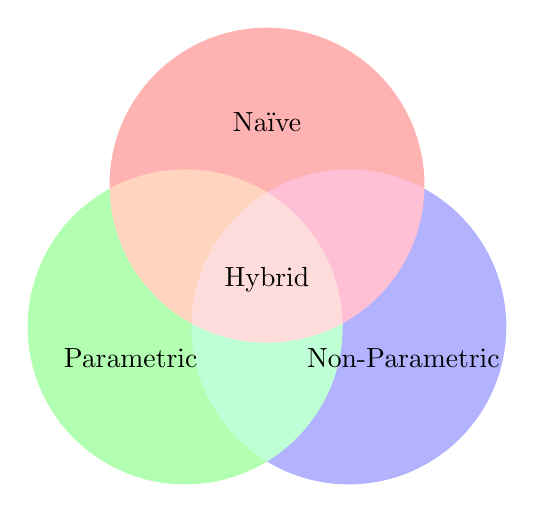
\begin{tikzpicture}
  \begin{scope}[blend group = soft light]
    \fill[red!30!white]   ( 90:1.2) circle (2);
    \fill[green!30!white] (210:1.2) circle (2);
    \fill[blue!30!white]  (330:1.2) circle (2);
  \end{scope}
  \node at (90:2)    {Naïve};
  \node at (210:2)   {Parametric};
  \node at (330:2)   {Non-Parametric};
  \node              {Hybrid};
\end{tikzpicture}
\caption{Methods used for short term traffic prediction} \label{fig:taxonomyTrafficPrediction}
\end{figure}

\section{Naïve methods}
These are heuristics methods, and often used in practice because of their simplicity and the ease
of implementations. In most cases these methods are used as baselines for comparison while
creating more advances methods. The simplest naive approach in short term prediction would be to
take the last observed value and this involves no computational effort. Another simple heuristic
method known as the historical averages uses the average of past observed values.

\section{Parametric models}
In parametric models, we estimate the parameters from the training dataset to determine the
function that classifies new unseen data. The number of parameters are fixed. The advantage of
parametric models are that these perform quite well in situations where the large amount of data
is not available. Some of the typical examples of parametric models include Linear and
nonlinear regression, ARIMA models, Kalman filter, Linear SVM etc.

\subsection{Classical regression}
In machine learning and statistical applications, the use of linear models are predominant. These
models are also important in time series domains such as traffic flow prediction. The primary
idea behind the regression is to express the output variable as a linear combination of input
vectors. We can express the linear regression in time series as an ouput influenced by a
collection of inputs, where the inputs could possibly be an independent series

        \begin{equation}
            x_{t} = \beta_{1}z_{t1} + \beta_{2}z_{t2} + ... + \beta_{q}z_{tq} + w_{t}
        \end{equation}

where $ \beta_{1}, \beta_{2},...,\beta_{q} $ are unknown regression coeffiecients and $w_{t}$ is
a random error.

\citet{hogberg1976estimation} used non-liner regression for traffic prediction.

\subsection{ARIMA}
%  Introduction to ARIMA models

ARIMA(Auto Regressive Integrated Moving Average) is a class of parametric regression models. In
this section we will introduce ARIMA and related methods such as exponential smoothing and moving
averages. For an in depth understanding of these models the reader is encouraged to refer to to
~\citet{tong1990non}, ~\citet{brockwell2006introduction} and ~\citet{box2015time}. It is
important to understand that ARIMA modelling works only with stationary time series data. A
stationary time series is one whose properties do not depend on the time it is being observed.
Trends and seasonality affect time series and hence make it non-stationary. Although this seems as a
big restriction, in short term traffic prediction, ARIMA models have been very successful. Two
basic models constituate ARIMA models - AR(autoregressive) and MA(moving average).

The main idea behind autoregressive models is that past values affect the present value, i.e.
$x_{t}$ can be expressed as a function of past p values $ x_{t-1}, x_{t-2},...,x_{t-p} $ , where
p is the number of steps into the past. We can express an autoregressive model of order p as below

        \begin{equation} \label{eq:autoregressive}
          x_{t} = \phi_{1}x_{t-1} + \phi_{2}x_{t-2} + ... + \phi_{p}x_{t-p} + w_{t}
        \end{equation}

where $x_{t}$ is stationary and $\phi_{1}, \phi_{2},..., \phi_{p}$ are constant
parameters that are to be chosen. We have added the term $w_{t}$ as a Guassian white noise with
zero mean and variance $\sigma^{2}_{w}$.

In the MA model, the current value is dependent on the last q one-step forecast errors
$e_{t-1}, e_{t-2},...,e_{t-q}$ and the white noise $w_{t}$. The expression for moving average
is

        \begin{equation} \label{eq:movingaverage}
          x_{t} = -\theta_{1}e_{t-1} - \theta_{2}e_{t-2} - ... - \theta_{q}e_{t-q} + w_{t}
        \end{equation}

$\theta_{1}, \theta_{2},..., \theta_{q}$ are the parameters to be chosen.

Now proceeding to an ARMA(autoregressive moving average) model, we define an ARMA(p,q) model
where the present value $x_{t}$ is dependent on p past recent values and q past recent forecast
errors and a white noise $w_{t}$.

        \begin{equation} \label{eq:arma}
          x_{t} = \phi_{1}x_{t-1} + \phi_{2}x_{t-2} + ... + \phi_{p}x_{t-p} - \theta_{1}e_{t-1}
          - \theta_{2}e_{t-2} - ... - \theta_{q}e_{t-q} + w_{t}
        \end{equation}

When q is 0, the model becomes an autoregressive model of order p, AR(p) and when p is 0 the model
is a moving average of order q, MA(q). We can rewrite \ref{eq:arma} by using the backshift
operator $B^{\alpha}$, which is defined as $B^{\alpha}z_{t} = z_{t-\alpha}$,

        \begin{equation} \label{eq:armarewrite}
          \phi(B)x_{t} = \theta(B)e_{t}
        \end{equation}

where
        \begin{equation}
            \phi(z) = 1 - \phi_{1}z - ... - \phi_{p}z^{p}
        \end{equation}
        \begin{equation}
            \theta(z) = 1 - \theta_{1}z - ... - \theta_{q}z^{q}
        \end{equation}

In practice, most time series data are non-stationary and so several approaches, for instance
by differencing, are taken to make it stationary before applying the ARMA(p,q) model. By
combining differencing with autoregressive and moving average we obtain the ARIMA model defined
as below
        \begin{equation} \label{eq:arima}
          x'_{t} = \phi_{1}x'_{t-1} + \phi_{2}x'_{t-2} + ... + \phi_{p}x'_{t-p} -
          \theta_{1}e_{t-1} - \theta_{2}e_{t-2} - ... - \theta_{q}e_{t-q} + w_{t}
        \end{equation}

where $x'_{t}$ is the differenced series. Formally the model is denotes as ARIMA(p,d,q) where p
is the order of autoregressive part, d is the degree of differencing and q is the order of moving
average. This is also known as a non-seasonal ARIMA model.

The common method used to determine the parameters in an ARIMA(p,d,q) model is known as the
Box-Jenkins approach (\citet{box2015time}) which is three stage procedure. The three stages are
identification, estimation and diagnostic checking. At the identification stage, the values p, d
and q are determined by observing the autocorrelation and partial autocorrelation functions of
the time series and its differences. At the estimation stage, the maximum liklihood estimates are
determined for each model parameter. Finally in the dignostics stage, the residuals are analysed
and model comparisions are done. If the model fits well then the standardised residuals behave as
an i.i.d. with mean zero and variance one.

% Application in traffic forecast
\citet{ahmed1979analysis} used Box-Jenkins method for short-term traffic forecast. The input data
used was 166 sets of time series traffic data collected by freeway traffic surveillance systems in
three locations - Los Angeles, Minneapolis and Detroit. The authors concluded an ARIMA(0,1,3)
model, based on the autocorrealtion and partial autocorrelation functions, as a resonable fit for
the short term prediction tasks for both traffic volume and occupancy. The model performance was
evaluated against a moving average, a double smoothing average and a Trigg and Leach adaptive
model. The comparisons suggest that the ARIMA model had better accuracy than the others. The
authors used this model in detecting traffic incidents by comparing the real-time flow occupancy
with the predicted value. \citet{nihan1980use} used the Box-Jenkins technique on monthly data
collected at 15 minutes interval on a freeway segment from 1968 to 1976 to forecast for the year
1977. After examining several models they finally selecte an ARIMA(12,1,7) model. The forecast
was done for average weekday volume with positive results.

\citet{williams2001multivariate} used an ARIMAX model to use upstream traffic data along with the
predicting location's traffic data while estimating the paramters of the ARIMA model. This is
done using ARIMAX model which is an extension of the ARIMA model where an exogenous variable is
used. The data was collected form four locations near Beaune, France. The data from three upstream
locations were used for forecasting at the fourth location in Beaune. The same data were used
in the proposed ATHENA and KARIMA models. The model was compared  against the univariate ARIMA,
ATHENA\citet{danech1991athena} and KARIMA(\citet{van1996combining}) models. The results show tha
the ARIMAX model consistently outperformed the ARIMA model. However the complexity of the ARIMAX
model is more than the ARIMA model with as many as twice the parameters to estimate. Also in case
of missing values the ARIMAX model performance degraded more than the ARIMA model.

\citet{min2009short} proposed a dynamic Space Time ARIMA (STARIMA) model for short term traffic
prediction. Their argument for the new proposed model was based on the factor that most of the
existed model failed to take the spatial information of the transporatation system into account.
The proposed dynamic STARIMA model combines STARIMA and Dynamic Turn Ratio Prediction (DTRP)
model. Using DTRP they dynamically updated the static matric $W_{k}$ in STARIMA model that contains
the structural information of the transporatation network. The results of the study showed
significant improvement in forecast accuracy. The authors later published another similar work
(\citet{min2010urban}) that used the generalised STARIMA (GSTARIMA) model.  The authors
presented the results where this model has a small improvements over the STARIMA model. However
the major drawbacks of the GSTARIMA model is the estimation of large number of parameters which
significantly increases the computational time. It also suffers in performance if enough historical
data is not available.

\citet{williams2003modeling} poposed for the acceptance of seasonal ARIMA models for short term
traffic prediction. A seasonal ARIMA $(p,d,q) (P,D,Q)_{s}$ for a time series {$x_{t}$} is one
where s is the period, d and D are nonnegative integers. The time series theorem known as the World
decomposition is used as the theoritical justification of applying seasonal ARIMA model to
univariate time series with stationarity. Data from two freeway locations, one each from the
United States and the United Kingdom were used for evaluating the model. The performance of the
models were compared against three heuristics approaches - historical averages, random walk and
deviation from historical avarages. The results show that for both the locations the seasonal
ARIMA has better performance than the three methods mentioned earlier. However the authors did
not present whether a non-seasonal ARIMA model would have similar performance. The only other
model that was considered for comparison was the KARIMA model, which did not perform as good as
the seasonal ARIMA model. \citet{kumar2015short} also used a seasonal ARIMA in the context of
limited data for short term traffic prediction. They used data collected over three days from an
arterial road in Chennai, India for the study. The model was validated on 24 hours ahead forecast
. Thier resluts were positive when compared with historical avereges and naïve methods. They
argued when availability of large traffic dataset is a constraint seasonal ARIMA method is a
better choice. \citet{szeto2009multivariate} used a hybrid SARIMA model with cell transmission
model for multivariate traffic prediction. The authors reasoned the use of multivariate models
captuered the spatial characteristics of the transporatation network and hence are the natural
and better choice over an univariate model. The model was validated against data collected form
the city center in Dublin, Ireland. The results at two junctions were compared against real
observations and had MAPE of 4.45 and 10.6. The authors however did not provide comparison
against other univariate models or multivariate models which could present the model's relative
performance.

% Conclusions - pros and cons
The major defficiency of tha ARIMA models is that they do not take the extremes into
consideration and focus on the means. This is in contrast to the nature of the traffic data.
ARIMA models are also have the inability to perform will with missing data as pointed out by
\citet{smith1997traffic}.


\subsection{Kalman filter}
Kalman filter is a paramteric regression technique usually used in the field of automatic control
systems and signal preocessing. It was proposed by \citet{kalman1960new}. It can be used on both
stationary and non-stationary time series.

\citet{okutani1984dynamic} used Kalman filtering in traffic prediction in an urabn network and
extended it for freeways.

\citet{wang2005real}

\citet{xie2007short}

\citet{guo2010real}

\citet{guo2014adaptive}

The main advantage of Kalman filtering is the state variable is updated continuously.

\subsection{Exponential smoothing}
In exponential smoothing method the forecast is the weighted average of past observations, while
the weights decrease exponentially for older observations. For time series data with no trends
and seasons single exponential smoothing is usually used.


\section{Non-Parametric models}
In nonparamtric models the parameters are not fixed, and vary with the amount of data available.
Usually more data is required for this models than parametric models. The advantage of these models
is that they can model the complex non-linear data better. Some of the widely used non-parametric
models are - k-Nearest Neighbour, Non-parametric regrssion and Neural Networks

\subsection{K-nearest neighbour}

The basic process of the k-nearest neighbour algorithm is described in figure \ref{fig:KnnProcessFlow}.


\tikzstyle{block} = [rectangle, draw, text width=5em, text centered, rounded corners,
minimum height=4em]
\tikzstyle{line} = [draw, -latex']
\tikzstyle{cloud} = [draw, ellipse, node distance=4cm, minimum height=3em]

\begin{figure}
\centering
\begin{tikzpicture}[node distance = 3cm, auto]
    % Place nodes
    \node [block] (pp) {Preprocess Data};
    \node [cloud, left of=pp] (hd) {Historical data};
    \node [cloud, right of=pp] (rd) {Real-time data};
    \node [block, below of=pp] (msv) {Match state vector};
    \node [block, below of=msv] (knn) {K nearest neighbour};
    \node [block, left of=knn, node distance=3cm] (prd) {Predictions};
    % Draw edges
    \path [line] (pp) -- (msv);
    \path [line] (msv) -- (knn);
    \path [line] (knn) -- (prd);
    \path [line,dashed] (hd) -- (pp);
    \path [line,dashed] (rd) -- (pp);
\end{tikzpicture}
\caption{K nearest neighbour process flow} \label{fig:KnnProcessFlow}
\end{figure}

\citet{lv2009real}

\citet{myung2011travel}

\citet{zhang2013improved}

\citet{meng2015two}


\subsection{Neural networks}
\label{subsec:neuralNetworksTrafficPred}
Artificial Neural Networks(ANN) were mathematical models (\citet{mcculloch1943logical},
\citet{rosenblatt1958perceptron}) designed to  provide a representation of how the human brain
works. It is obvious now that these mathematical models bear little resemblance to the structure
of brain, yet they have been hugely successful. Because they were initially inspired by the
biological brain, the term neural is associated with such kind of mathematical models. A basic
artificial neural network consists of a set of nodes connnected by edges with weights. We can say
that the nodes represent the biological neurons and the edges represent the synapses. The
conections among the nodes can be cyclic or acyclic. The former is known as a feedforward neural
network and the later as a recurrent network. We describe about these neural networks in more
details in chpater \ref{Chapter4}. Several variations of artificial neural networks have been
used in short term traffic prediction. Some well known examples include - \textit{Multilayer
perceptrons, Radial basis function networks, Kohnen maps} and \textit{Hopfield networks}.

\cite{dougherty1997short} apllied a backpropagation feedforward neural network in traffic flow
and speed predictions.

\subsection{Fuzzy logic}

\cite{zhang2008short}

\subsection{Bayesian networks}

\cite{castillo2008predicting}


\section{Hybrid Methods}
In recent years many hybrid methods have been tried in short term traffic prediction with mixed
results.

A hybrid method by combining kohonen maps with ARIMA model was proposed by \citet{van1996combining}.
The model known as KARIMA, used the same data(collected near Beaune, France) that was used in the
ATHENA model for an accurate comparison with the later.

\citet{chen2011short} proposed an ARIMA-GARCH model for short term traffic prediction. The
performance of this hybrid model when compared to the standard ARIMA model did not yield positive
results.

\section{Comparisons}

% Chapter 3

\chapter{SCATS Volume Data} % Main chapter title

% For referencing the chapter elsewhere, use \ref{Chapter3}
\label{Chapter3}

% This is for the header on each page - perhaps a shortened title
\lhead{Chapter 3. \emph{SCATS Volume Data}}

%----------------------------------------------------------------------------------------
% Quotation
``There is no order in the world around us, we must adapt ourselves to the requirements of chaos
instead."

\begin{flushright}
Kurt Vonnegut, \textit{Breakfast of Champions} (1973)
\end{flushright}

%---------------------------------------------------------------------------------------------------
%	CONTENT
%   Reference - http://www.scats.com.au/files/an_introduction_to_scats_6.pdf
%---------------------------------------------------------------------------------------------------
\section{Introduction}
SCATS(Sydney Coordinated Adaptive Traffic System) is an adaptive traffic control system. It was
developed by the Department of Main Roads in the 1970's. SCATS operates in real-time by adjusting
signal timings in response to changes in traffic demand and road capacity. All major and minor
cities in Australia and New Zealand use SCATS. Few other cities around the world such as Hong
Kong, Kuala Lumpur, Sanghai and Singapore also have adopted SCATS over other adaptive traffic
control system. In Melbourne and surrounding cities, SCATS controls more than 3,900 sets of traffic
signals

There are three main parameters that SCATS user to achieve traffic signal coordination:
\begin{itemize}
\item[\tiny{$\blacksquare$}] Cycle time: The total time of all signal sequences in a cycle
\item[\tiny{$\blacksquare$}] Phase split: The proportion of the cycle time allocated to each phase
\item[\tiny{$\blacksquare$}] Offset: The time relationship between the starting and finishing of
the green phases of succesive sets of signals within a coordinated system
\end{itemize}

The desicion making of the SCATS system occurs at two levels - \emph{strategic} and \emph{tactical}.


\section{Volume data}
Traffic loop detectors are embedded in the raod pavement and located in each lane near the stop
line at traffic intersections. These detectors collect traffic volume and the time it takes a
vehicle to clear the loop.


\subsection{Handling missing data}


\section{Exploratory analysis}
Figure \ref{fig:AverageTrafficVolume} shows the daily, weekly, monthly and yearly average traffic
volume at a site
location.

\begin{figure}[htbp]
  \centering
    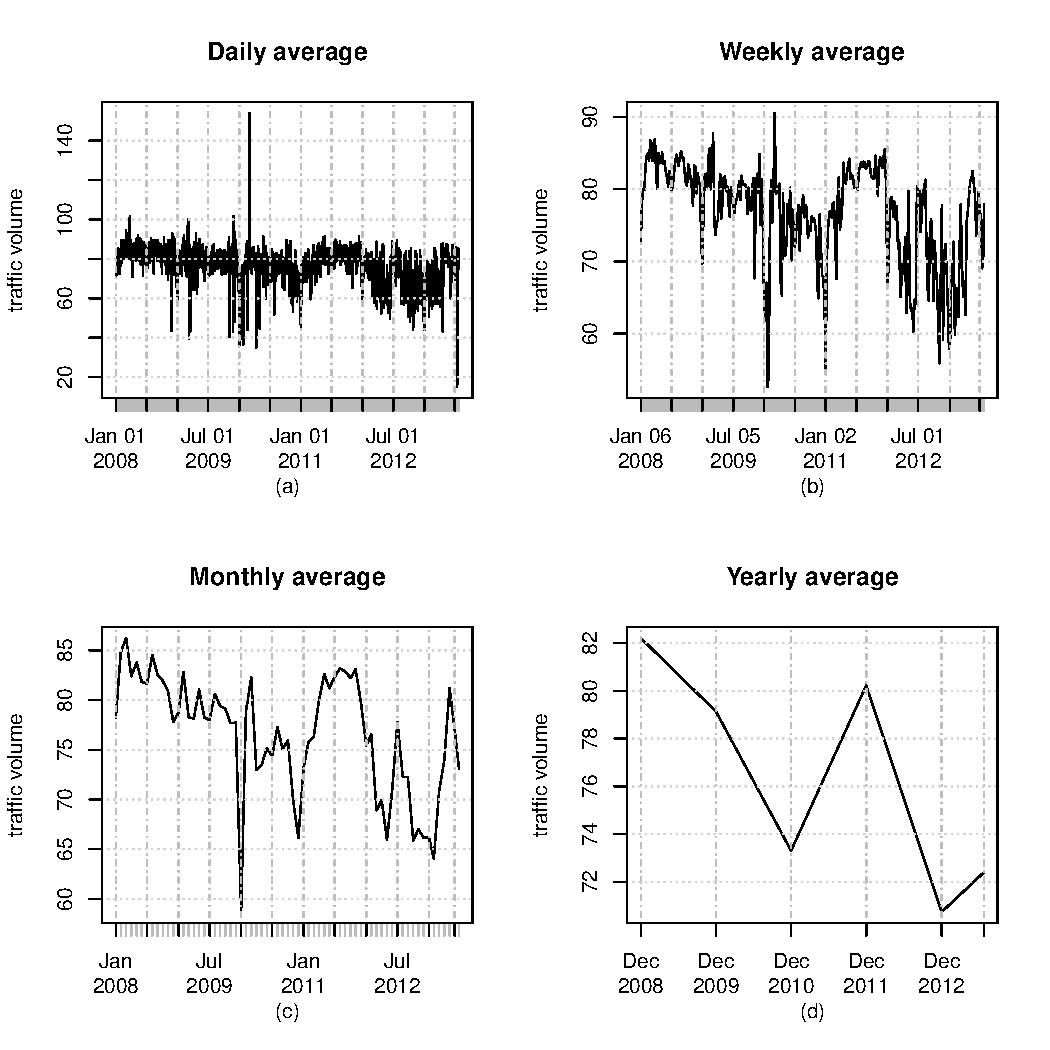
\includegraphics[width=\textwidth,height=\textheight,keepaspectratio]{Figures/averages.pdf}
    \rule{35em}{0.5pt}
  \caption[Average Traffic Volume]{(a) daily, (b) weekly, (c) monthly and (d) yearly average of
  traffic volume (15 mins interval) at a site location from the period 01/01/2008 to 26/07/2013}
  \label{fig:AverageTrafficVolume}
\end{figure}

% Chapter 4

\chapter{A Deep Recurrent Network Model for Traffic Flow Prediction} % Main chapter title

\label{Chapter4} % For referencing the chapter elsewhere, use \ref{Chapter4}

% This is for the header on each page - perhaps a shortened title
\lhead{Chapter 4. \emph{A Deep Recurrent Network Model for Traffic Flow Prediction}}

% Quotation
{``I am a brain, Watson. The rest of me is a mere appendix."}
\begin{flushright}
Arthur Conan Doyle, \textit{The Adventure of the Mazarin Stone} (1921)
\end{flushright}

%---------------------------------------------------------------------------------------------------
%	CONTENT
%---------------------------------------------------------------------------------------------------

\section{Introduction}
Today we live in a world where almost every interaction of ours with the external world uses some
form of computing. Computers have become an inseparable part of human lives. In the earlier days
when computers were built, people began to ponder whether they could achieve human level
of intelligence. Even though at that point the answers seemed optimistic, it has taken quite
some time and understanding on our part to make significant achievements in the field of
artificial intelligence. One of the approaches was to use knowldge base systems, where computers
reason about real world concepts, that were defined in hard-coded formal langauges, using logical
inference rules. These systems led to little success. The difficulties faced in the knwoledge
based appproach made us built computers to learn automatically from data, an approach we know as
machine learning. A large number of real world problems could eaily be tackled using machine
leraning. However for the machine learning algorithms to perorm well they need to be provided
with proper representaion of data. For example <TODO - an exmple of representaion>

Finding a proper representation from data is a challenge and sometimes become very difficult.

<TODO - Deep learning>

\section{Recurrent neural networks}

\subsection{LSTM Networks}
In previous section we learn that using a recurrent neural networks we can store information in
form of activations in the feedback connnections.

% Chapter 5

\chapter{Evaluation of the Model} % Main chapter title

\label{Chapter5} % For referencing the chapter elsewhere, use \ref{Chapter5}

% This is for the header on each page - perhaps a shortened title
\lhead{Chapter 5. \emph{Evaluation of the Model}}

% Quotation
``Science, my boy, is made up of mistakes, but they are mistakes which it is useful to make,because
they lead little by little to the truth"

\begin{flushright}
Jules Verne, \textit{Journey to the Centre of the Earth} (1864)
\end{flushright}

%---------------------------------------------------------------------------------------------------
%	CONTENT
%---------------------------------------------------------------------------------------------------

\section{Experimental setup}
%1892 VICTORIA STREET 12607 W BD 16911
%1893 VICTORIA STREET 12608 W BD 16912
%1897 VICTORIA STREET 12612 W BD 16913
% Hoddle st - 268 to 278 (South bound)
% Hoddle st - 10522 to 16517 (North bound)
% Bridge Road 14475 - 14479 (West bound)
% Barkers Road 16548 - 16551 (West bound)
% Princess st 6297 (South bound)
% Power st - 16537 - 16538 (North bound)

\subsection{Training details}
We trained our stacked LSTM network(\ref{sec:stackedLSTMTrafficPred})

\section{Results}

For comparison purose we used the following methods that have been in used predominantly in short
term traffic prediction - Naïve, Linear regression, ARIMA, Exponential smoothing and Feedforward
neural network. In figure \ref{fig:benchmarkModels}, we present the predictions of these models
on test data. The input sequence was set to 96 observations(1 day) and the prediction was done for
next 15 minutes(1 step ahead).


\begin{figure}[h]
    \centering

    \subfloat[Naïve][Naïve]{
    \includegraphics[width=0.4\textwidth]{Plots/naive1.pdf}
    \label{fig:naive1ActualPredicted}}

    \subfloat[Linear Regression][Linear Regression]{
    \includegraphics[width=0.4\textwidth]{Plots/linear1.pdf}
    \label{fig:lm1ActualPredicted}}
    \qquad
    \subfloat[ARIMA][ARIMA]{
    \includegraphics[width=0.4\textwidth]{Plots/arima1.pdf}
    \label{fig:arima1ActualPredicted}}

    \subfloat[Exponential smoothing state space model][Exponential smoothing state space model]{
    \includegraphics[width=0.4\textwidth]{Plots/ets1.pdf}
    \label{fig:ets1ActualPredicted}}
    \qquad
    \subfloat[Neural Network AutoRegression][Neural Network AutoRegression]{
    \includegraphics[width=0.4\textwidth]{Plots/nnetar1.pdf}
    \label{fig:nnetar1ActualPredicted}}

    \caption[Acutual vs Predictions, using currently popular methods]{Acutual vs Predictions -
    linear regression, ARIMA, feed forward neural network one hidden layer and exponential
    smoothing using state space model. The models were trained on trafiic data from one homogeneous
    road segment. The plots show the actual vs predictions(15 mins) on 400 test examples, for one
    of those road segment (Nicholson street between Gertrude street and Victoria Parade).}
    \label{fig:benchmarkModels}
\end{figure}

The results of the LSTM network are shown in the figure \ref{fig:LSTMActualPredicted}

\begin{figure}[h]
    \centering


    \subfloat[K-Nearest Neighbour][K-Nearest Neighbour]{
    \includegraphics[width=0.4\textwidth]{Plots/knn1.pdf}
    \label{fig:knn1ActualPredicted}}
    \qquad
    \subfloat[Support Vector Regression][Support Vector Regression]{
    \includegraphics[width=0.4\textwidth]{Plots/svm1.pdf}
    \label{fig:svm1ActualPredicted}}

    \subfloat[LSTM - single location][LSTM - single location]{
    \includegraphics[width=0.4\textwidth]{Plots/lstm-single1.pdf}
    \label{fig:LSTMActualPredicted1}}
    \qquad
    \subfloat[GRU - single location][GRU - single location]{
    \includegraphics[width=0.4\textwidth]{Plots/gru1.pdf}
    \label{fig:GRUActualPredicted1}}

    \subfloat[RNN - single location][RNN - single location]{
    \includegraphics[width=0.4\textwidth]{Plots/rnn1.pdf}
    \label{fig:RNNActualPredicted1}}
    \qquad
    \subfloat[LSTM - multiple locations][LSTM - multiple locations]{
    \includegraphics[width=0.4\textwidth]{Plots/lstm-multi1.pdf}
    \label{fig:LSTMMultiActualPredicted1}}

    \caption[Acutual vs Predictions, using deep LSTM networks]{Acutual vs Predictions - The left
    figure is from the model trained using data from a single homogeneous road segment only. The
    figure in right is from the model trained on 67 homogeneous road segements in the chosen
    subnetwork(\ref{fig:ExperimentRegion}). Both the plots show the actual vs predictions(15
    mins) on 400 test examples, for one of those road segment(Nicholson street between Gertrude
    street and Victoria Parade).}
    \label{fig:LSTMActualPredicted}
\end{figure}

In table \ref{table:accuracyScores}, the performance of the LSTM network along with the compared
models are given.

Several accuracy measures exist to evaluate a model. In below secions we describe
the accuracy mesures and use those to evalute our proposed model against the benchmark models.
For defining the accuracy measures let us denote $x_{i}$ be the $i^{th}$ observation and
$\hat{x}_{i}$ be the prediction of $x_{i}$.

\textbf{Scale-dependent errors}
The prediction error is simply given by $e_{i} = x_{i} - \hat{x}_{i}$, which is in the same scale
as of the original data. So accuracy measures that depend on $e_{i}$ are scale dependent and can
not be used across multiple series on different scales. The two most used scale-dependent
accuracy measures are mean absolute error and root mean squared error defined as below

    \begin{equation}
        MAE = mean(\abs{e_{i}})
    \end{equation}
    \begin{equation}
        RMSE = \sqrt{mean(e^{2}_{i})}
    \end{equation}

MAE is easy to understand and popular in usage when using a single dataset.

\textbf{Percentage errors}
Percentage errors are scale-independent and thus used across multiple datasets on different
scales. The percentage error is given by $p_{i} = 100*e_{i}/x_{i}$. The most commonly used
percentage measure is Mean Absolute Percentage Error(MAPE) which is given by the below formula
    \begin{equation}
        MAPE = mean(\abs{p_{i}})
    \end{equation}

There are however few shortccomings of the MAPE, for instance when $x_{i}$ is 0 or very large.
Another shortcoming is that they put heavier penalty on negative error values than positve error
values.

\textbf{Scaled errors}
\citet{hyndman2006another} proposed scaled errors to be used as an alternative in place of
percentage errors. The proposed Mean Absolute Scaled Error(MASE) is defined as

    \begin{equation}
        MASE = mean(\abs{q_{i}})
    \end{equation}

where
    \begin{equation}
        q_{i} = \frac{e_{i}}{\frac{1}{T-1} \displaystyle\sum_{t=2}^{T}\abs{x_{t} - x_{t-1}}}
    \end{equation}

A scaled error is less than one if it is better than the average naïve forecast computed on the
training data and vice versa.

\begin{table}
    \begin{tabular}{c}
        \includegraphics[width=\textwidth,height=\textheight,keepaspectratio]{Figures/errors-table.pdf}
    \end{tabular}
    \caption[Model comparisons]{Accuracy measures for the evaluted models. The scores are
    calculated for prediction horizon of 15-minutes and 30-minutes. Mean 15-minutes traffic
    volume is 224.1}
    \label{table:accuracyScores}
\end{table}

% Chapter 6

\chapter{Conclusions and Future Directions} % Main chapter title

\label{Chapter6} % For referencing the chapter elsewhere, use \ref{Chapter6}

% This is for the header on each page - perhaps a shortened title
\lhead{Chapter 6. \emph{Conclusions and Future Directions}}

% Quotation
``Everything should be made as simple as possible but not simpler."

\begin{flushright}
Albert Einstein
\end{flushright}


%---------------------------------------------------------------------------------------------------
%	THESIS CONTENT - APPENDICES
%---------------------------------------------------------------------------------------------------

\addtocontents{toc}{\vspace{2em}} % Add a gap in the Contents, for aesthetics

\appendix % Cue to tell LaTeX that the following 'chapters' are Appendices

% Include the appendices of the thesis as separate files from the Appendices folder Uncomment the
% lines as you write the Appendices

\input{Appendices/AppendixA}
%\input{Appendices/AppendixB}
%\input{Appendices/AppendixC}

\addtocontents{toc}{\vspace{2em}} % Add a gap in the Contents, for aesthetics

\backmatter

%---------------------------------------------------------------------------------------------------
%	BIBLIOGRAPHY
%---------------------------------------------------------------------------------------------------

\label{Bibliography}

\lhead{\emph{Bibliography}} % Change the page header to say "Bibliography"

\bibliographystyle{apalike} % Use the "apalike" BibTeX style for formatting the Bibliography

% The references (bibliography) information are stored in the file named "Bibliography.bib"
\bibliography{Bibliography}

\nocite{*}

\end{document}
